\documentclass[11pt, oneside]{article}
\usepackage{geometry}
\usepackage{amsmath}
\geometry{letterpaper}

%verbatim environments
\usepackage{verbatim}
\usepackage{fancyvrb}
\DefineVerbatimEnvironment{printout}{Verbatim}{fontsize=\small}

%semantic package (with inference)
\usepackage[inference, reserved]{semantic}

%%% Diagram drawing
\usepackage{tikz}
\usetikzlibrary{arrows,automata,calc,shapes, positioning}
%% math
\newcommand{\set}[1]{\{#1\}}

%% LTLf/LDLf
\let\vphi\varphi % alternate phi, which I'll be using a lot
\newcommand{\di}[1]{\langle#1\rangle} % 'diamond' For LDL modalities
\newcommand{\sq}[1]{[#1]} % 'square'
\newcommand{\luntil}{\ \mathcal{U}\ }
\newcommand{\lalways}{\mathcal{G}}
\newcommand{\leventually}{\mathcal{F}}
\newcommand{\lnext}{\circ\,}
\newcommand{\prog}{\Pi}
\newcommand{\A}{\mathnormal{A}}
\newcommand{\prop}{\mathcal{P}}
\newcommand{\actions}{\mathcal{A}}
\newcommand{\fin}[1]{#1$_f$}
\newcommand{\ltlf}{LTL$_f\ $}
\newcommand{\ldlf}{LDL$_f\ $}

\begin{document}

\newcommand{\ldlfa}{LDL$_f$}
\newcommand{\ldlfb}{LDL$_f\,$}
\ldlf. \ldlf blah.
\\\ldlfa. \ldlfa blah.
\\\ldlfb. \ldlfb blah.
%
{\newcommand{\lab}{$\lnext$}
\begin{figure}
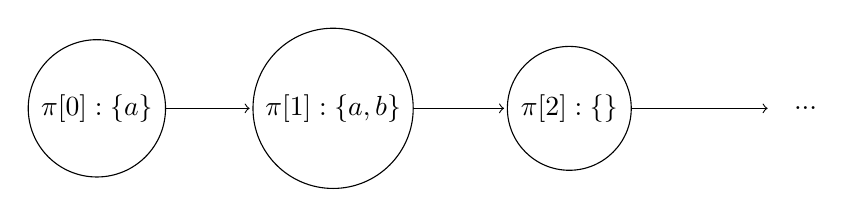
\begin{tikzpicture}[shorten >=1pt,node distance=3cm,on grid,auto]
   \node[state] (q1)   {$\pi[0]: \set{a}$};
   \node[state] (q2) [right=of q1] {$\pi[1]: \set{a,b}$};
   \node[state] (q3) [right=of q2] {$\pi[2]: \set{}$};
   \node[state, draw=none] (q4) [right=of q3] {...};
    \path[->]
    (q1) edge node {\lab} (q2)
    (q2) edge node {\lab} (q3)
    (q3) edge node {\lab} (q4);

\end{tikzpicture}
    \caption{Diagram of an infinite trace\label{fig:inf_trace_diagram}}
\end{figure}
}

%
\usetikzlibrary{shapes,shapes.geometric,arrows,fit,calc,positioning,automata,}
\tikzset{rectangular state/.style={draw,rectangle,minimum width=1cm,minimum height=1cm}}

\begin{figure}
\begin{printout}
====================================================================================================
LDL: <(<(True;True)>a?;True)*>b
------------------------------------------------------------
AFA: Alphabet: {{}, {a}, {a, b}, {b}}
States: {a, <True>a, <(<(True;True)>a?;True)*>b}
Init: <(<(True;True)>a?;True)*>b
Transition: a X {} -> False
a X {a} -> True
a X {a, b} -> True
a X {b} -> False
<True>a X {} -> state(a)
<True>a X {a} -> state(a)
<True>a X {a, b} -> state(a)
<True>a X {b} -> state(a)
<(<(True;True)>a?;True)*>b X {}
  -> (False || (state(<True>a) && state(<(<(True;True)>a?;True)*>b)))
<(<(True;True)>a?;True)*>b X {a}
  -> (False || (state(<True>a) && state(<(<(True;True)>a?;True)*>b)))
<(<(True;True)>a?;True)*>b X {a, b}
  -> (True || (state(<True>a) && state(<(<(True;True)>a?;True)*>b)))
<(<(True;True)>a?;True)*>b X {b}
  -> (True || (state(<True>a) && state(<(<(True;True)>a?;True)*>b)))

Final: {}
\end{printout}
\caption{Printout of ``Until'' formula results (AFA) \label{fig:until_printout_afa}}
\end{figure}
\begin{figure}
  \begin{printout}
------------------------------------------------------------
NFA: Alphabet: {{}, {a}, {a, b}, {b}}
States: {{}, {a}, {a, <True>a, <(<(True;True)>a?;True)*>b},
{<True>a, <(<(True;True)>a?;True)*>b}, {<(<(True;True)>a?;True)*>b}}
Init: {<(<(True;True)>a?;True)*>b}
Transition: {} X {} -> {{}}
{} X {a} -> {{}}
{} X {a, b} -> {{}}
{} X {b} -> {{}}
{a} X {} -> {}
{a} X {a} -> {{}}
{a} X {a, b} -> {{}}
{a} X {b} -> {}
{a, <True>a, <(<(True;True)>a?;True)*>b} X {} -> {}
{a, <True>a, <(<(True;True)>a?;True)*>b} X {a} -> {{a, <True>a, <(<(True;True)>a?;True)*>b}}
{a, <True>a, <(<(True;True)>a?;True)*>b} X {a, b} -> {{a}}
{a, <True>a, <(<(True;True)>a?;True)*>b} X {b} -> {}
{<True>a, <(<(True;True)>a?;True)*>b} X {} -> {{a, <True>a, <(<(True;True)>a?;True)*>b}}
{<True>a, <(<(True;True)>a?;True)*>b} X {a} -> {{a, <True>a, <(<(True;True)>a?;True)*>b}}
{<True>a, <(<(True;True)>a?;True)*>b} X {a, b} -> {{a}}
{<True>a, <(<(True;True)>a?;True)*>b} X {b} -> {{a}}
{<(<(True;True)>a?;True)*>b} X {} -> {{<True>a, <(<(True;True)>a?;True)*>b}}
{<(<(True;True)>a?;True)*>b} X {a} -> {{<True>a, <(<(True;True)>a?;True)*>b}}
{<(<(True;True)>a?;True)*>b} X {a, b} -> {{}}
{<(<(True;True)>a?;True)*>b} X {b} -> {{}}

Final: {{}}

------------------------------------------------------------
Satisfiable? According to NFA's final state set, yes
====================================================================================================
\end{printout}
\caption{Printout of ``Until'' formula results (NFA) \label{fig:until_printout_nfa}}
\end{figure}

{
\newcommand{\rhoY}{\di{true;true}a?}
\newcommand{\rhoX}{\di{true;true}a?;true}
\begin{figure}
\begin{tikzpicture}[shorten >=1pt,node distance=2cm,on grid,auto]
  \node[rectangular state] (RXSTARB) {$\di{(\rhoX)^*}b$};
  \node[rectangular state] (B) [right of = RXSTARB, node distance = 6 cm] {$b$};
  \node[rectangular state] (RXRXSTARB) [below of = RXSTARB] {$\di{\rhoX}\di{(\rhoX)^*}b$};
  \node[rectangular state] (RYTRXSTARB) [below of = RXRXSTARB] {$\di{\rhoY}\di{true}\di{(\rhoX)^*}b$};
  \node[rectangular state] (TRXSTARB) [right of = RYTRXSTARB, node distance = 8 cm ] {$\di{true}\di{(\rhoX)^*}b$};
  \node[rectangular state] (T) [below right of = TRXSTARB, node distance = 4 cm] {$true$};
  \node[rectangular state] (TTA) [below of = RYTRXSTARB] {$\di{true;true}a$};
  \node[rectangular state] (A) [right of = TTA, node distance = 6 cm] {$a$};
  \node[rectangular state] (TTA2) [below of = TTA] {$\di{true}\di{true}a$};
  \node[rectangular state] (TA) [right of = TTA2, node distance = 6 cm] {$\di{true}a$};
  \path[->]
  (RXSTARB) edge [blue, bend left] node [sloped, above] {formula} (B)
            edge node {star} (RXRXSTARB)
  (RXRXSTARB.0) edge [blue, bend right] node [sloped, above] {formula} (RXSTARB)
  (RXRXSTARB)   edge node {concat} (RYTRXSTARB)
  (RYTRXSTARB) edge [blue] node {formula} (TRXSTARB)
                edge node {test} (TTA)
  (TRXSTARB) edge [blue, bend right] node [sloped, above] {formula} (RXSTARB)
              edge [green] node {propositional} (T)
  (TTA) edge [blue] node {formula} (A)
        edge node {concat} (TTA2)
  (TTA2) edge [blue] node {formula} (TA)
      edge [green, bend right] node [sloped, above] {propositional} (T)
  (TA) edge [blue] node {formula} (A)
      edge [green] node [sloped, above] {propositional} (T);
\end{tikzpicture}
\caption{Fisher-Ladner closure of formula $\di{(\di{true;true}a?;true)^*}b$
(not the showing negated formulae-- of which there are exactly one for each shown)} \label{fig:until_fl}
\end{figure}
}
\begin{figure}
\begin{tikzpicture}[shorten >=1pt,node distance=2cm,on grid,auto]
   \node[initial, rectangular state] (q1)   {$q_1$: $\di{(\di{true;true}a?;true)^*}b$};
   \node[rectangular state] (q2) [above right of= q1, node distance = 6 cm] {$q_2$: $\di{true}a$};
   \node[rectangular state] (q3) [below right of= q2, node distance = 6 cm] {$q_3$: $a$};
   \node[state, draw=none, green] (true) [below of=q3] {True};
   \node[state, draw=none, red] (false) [left of = q3, node distance = 3.2 cm] {False};
   \node[state, magenta] (and) [right of = q1, node distance = 4 cm] {$\land$};
   \node[state, blue] (orFalse) [above right of = q1, node distance = 4 cm] {$\lor$};
   \node[state, blue] (orTrue) [below right of = and, node distance = 3 cm] {$\lor$};


    \path[->]
    (q3) edge node [sloped, above] {$\set{}, \set{b}$} (false)
         edge node {$\set{a}, \set{a,b}$} (true)
    (q2) edge node [sloped, above] {$\set{}, \set{a}, \set{b}, \set{a,b}$} (q3)
    (q1) edge node [sloped, above] {$\set{}, \set{a}$} (orFalse)
         edge node [align=center, sloped, above] {$\set{b}, \set{a,b}$} (orTrue)
    (and) edge node {} (q1)
          edge node {} (q2)
    (orFalse) edge node {} (and)
              edge node {} (false)
    (orTrue)  edge node {} (and)
              edge node {} (true);
\end{tikzpicture}
\caption{AFA constructed from formula (note that the states are a subset of the Fisher-Ladner closure)}\label{fig:until_afa}
\end{figure}


\begin{figure}
\begin{tikzpicture}[shorten >=1pt,node distance=2cm,on grid,auto]
   \node[initial, rectangular state] (q1)   {$q_1$: $\di{(\di{true;true}a?;true)^*}b$};
   \node[state, magenta] (and) [above right of = q1, node distance = 5 cm] {$\land$};
   \node[rectangular state] (q2) [right of= and, node distance = 4 cm] {$q_2$: $\di{true}a$};
   \node[rectangular state] (q3) [below of= q2, node distance = 4 cm] {$q_3$: $a$};
   \node[state, draw=none, green] (true) [below left of=q3, node distance = 4 cm] {True};
   \node[state, draw=none, red] (false) [left of = q3, node distance = 3.2 cm] {False};


    \path[->]
    (q3) edge node [sloped, above] {$\set{}, \set{b}$} (false)
         edge node [sloped, above] {$\set{a}, \set{a,b}$} (true)
    (q2) edge node {$\set{}, \set{a}, \set{b}, \set{a,b}$} (q3)
    (q1) edge [bend right] node [sloped, above] {$\set{}, \set{a}$} (and.315)
         edge node [sloped, above] {$\set{b}, \set{a,b}$} (true)
    (and) edge [bend right] node [align=center] {} (q1)
    (and)      edge node {} (q2);
\end{tikzpicture}
\caption{Simplified version of figure \ref{fig:until_afa}}\label{fig:until_afa_simp}
\end{figure}

%\begin{figure}
\begin{framed}
\begin{center}
Propositional:
\\\mbox{
  \inference[init]{}{\vphi} (original)
  $\quad$ \inference[negation]{\psi}{\neg\psi} (if $\psi$ not of the form $\neg\psi'$)
  $\quad$ \inference[conjunction]{\vphi_1 \land \vphi_2}
                          {\vphi_1, \vphi_2}
}
\\Modalities (base):
\\\mbox{
  \inference[formula]{\di{\rho}\vphi}{\vphi}
  $\quad$ \inference[propositional]{\di{\phi}\vphi}{\phi} ($\phi$ propositional)
  $\quad$ \inference[test]{\di{\psi?}\vphi}{\psi}
}
\\Modalities (inductive):
\\\mbox{
  \inference[concatenation]{\di{\rho_1;\rho_2}\vphi}{\di{\rho_1}\di{\rho_2}\vphi}
  $\quad$ \inference[addition]{\di{\rho_1 + \rho_2}\vphi}{\di{\rho_1}\vphi, \di{\rho_2}\vphi}
  $\quad$ \inference[star]{\di{\rho^*}\vphi}{\di{\rho}\di{\rho^*}\vphi}
}
\end{center}
\end{framed}
\caption{Fisher-Ladner closure of $\vphi$. Note that some rules have multiple
outputs (e.g. conjunction).\label{fig:fisher_ladner_closure}}

\end{figure}


$\delta(A, \Pi) = true \text{ if } A \in \Pi$
\\
$ \begin{displaystyle}
\delta(\di{\phi}\vphi, \Pi) = \left.
\begin{cases}
\vphi & \text{if } \Pi \models \phi \text{($\phi$ propositional)}\\
false & \text{if } \Pi \not\models \phi
\end{cases}

\end{displaystyle}$


\end{document}
